\documentclass[a4paper,10pt, leqno]{article}
\usepackage[utf8]{inputenc}
\usepackage{mathtools}
\usepackage{amsfonts}
\usepackage{amssymb}
\usepackage{amsthm}
\usepackage{graphicx}
\usepackage{indentfirst}
\usepackage{array}
\usepackage{bm}
\usepackage{caption}
\usepackage{algorithm}
\usepackage[noend]{algpseudocode}
\usepackage{bbm}
%\usepackage{algorithmic}

\newcommand{\restr}[1]{|_{#1}}

\theoremstyle{definition}
\def\blankpage{%
      \null%
      \clearpage}

\let\oldref\ref
\renewcommand{\ref}[1]{(\oldref{#1})}

%opening
\title{MAC0325 Combinatorial Optimization \\
        \large Assignment 2 }
\author{Pedro Gigeck Freire \\
        10737136}
\date{November 12, 2020}

%\setlength{\parindent}{0.5em}
%\setlength{\parskip}{0.1em}
\begin{document}

\maketitle


\section*{Exercise 1}
At each iteration $t$ we will show the path $P_t$ taken at line 11 of the algorithm (without showing the arcs).

\bgroup
\def\arraystretch{1.8}
\begin{center}
\begin{tabular}{|m{0.4cm}|m{3cm}|}
\hline 
\centering $\bm{t}$ & \centering\arraybackslash $\bf{P_t}$ \\ 
\hline 
\centering $1$ & \centering\arraybackslash $\langle r, a, c, s \rangle$ \\
\hline 
\centering $2$ & \centering\arraybackslash $\langle r, a, d, s \rangle$ \\
\hline 
\centering $3$ & \centering\arraybackslash $\langle r, p, b, s \rangle$ \\
\hline 
\centering $4$ & \centering\arraybackslash $\langle r, q, d, s \rangle$ \\
\hline 
\centering $5$ & \centering\arraybackslash $\langle r, a, c, b, s \rangle$ \\
\hline
\centering $6$ & \centering\arraybackslash $\langle r, p, q, b, s \rangle$ \\
\hline
\centering $7$ & \centering\arraybackslash $\langle r, a, c, q, d, s \rangle$ \\
\hline
\end{tabular}
\end{center}
\egroup

At the end of the execution, the $rs$-flow $f$ found is ilustrated in figure 1.1, and explicited below. The value of $f$ is $17$.

\bgroup
\def\arraystretch{1.8}
\begin{center}
\begin{tabular}{|m{0.8cm}|m{0.8cm}|m{0.8cm}|m{0.8cm}|m{0.8cm}|m{0.8cm}|m{0.8cm}|m{0.8cm}|m{0.8cm}|}
\hline 
\centering $\bf{a}$ 
& $(r, p)$
& $(r, a)$
& $(r, q)$
& $(p, q)$
& $(q, p)$
& $(p, b)$
& $(q, b)$
& $(q, d)$
\\ \hline
$\bf{f(a)}$ 
& \centering $5$
& \centering $8$
& \centering $4$
& \centering $2$
& \centering $0$
& \centering $3$
& \centering $0$
& \centering\arraybackslash $5$
\\ \hline
\end{tabular}
\end{center}
\egroup

\bgroup
\def\arraystretch{1.8}
\begin{center}
\begin{tabular}{|m{0.8cm}|m{0.8cm}|m{0.8cm}|m{0.8cm}|m{0.8cm}|m{0.8cm}|m{0.8cm}|m{0.8cm}|m{0.8cm}|}
\hline 
$(b, a)$
& $(a, c)$
& $(a, d)$
& $(c, q)$
& $(c, b)$
& $(d, c)$
& $(d, s)$
& $(c, s)$
& $(b, s)$
\\ \hline
\centering $0$
& \centering $7$
& \centering $1$
& \centering $1$
& \centering $2$
& \centering $0$
& \centering $6$
& \centering $4$
& \centering\arraybackslash $7$
\\ \hline
\end{tabular}
\end{center}
\egroup

The set $R$ that solves the minimum $rs$-cut problem is $R \coloneqq \{r, a, c, p \}$. It is ilustrated in figure 1.2.

\begin{figure}[ht]
\centering
  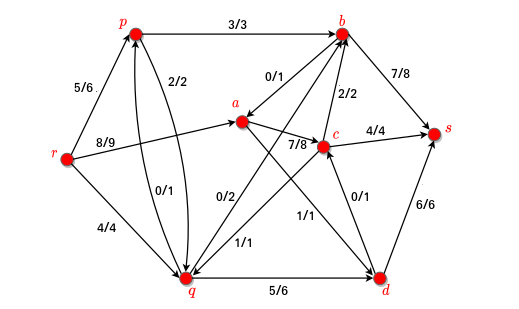
\includegraphics[width=30em]{flow.png}
  \captionsetup{labelformat=empty}
  \caption{Figure 1.1: $rs$-flow returned by the algorithm}
\end{figure}
\begin{figure}[ht]
\centering
  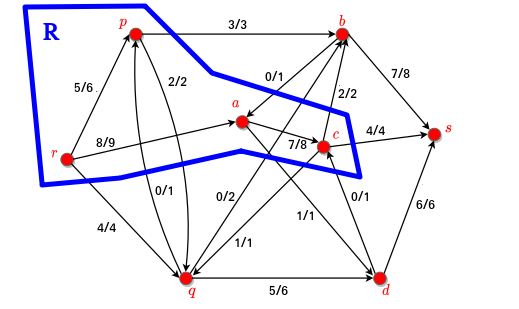
\includegraphics[width=30em]{cut.png}
  \captionsetup{labelformat=empty}
  \caption{Figure 1.2: $rs$-cut $R$ returned by the algorithm}
\end{figure}

\blankpage

\section*{Exercise 5}
\newtheorem{proposition}{Proposition}

\begin{proposition}
    Restore the context from the exercise statement. Let $f$ be an optimal solution for  the maximum flow problem with input $(D, u, r, s)$, let $R$ be an optimal solution for $(4.1)$ with the same input, i.e., a minimum $rs$-cut. Then 
    \begin{align*}
     f(a) &= u(a) \text{ for each } a \in \delta^{\text{out}}(R) \text{ and} \\
     f(a) &= 0 \text{ for each } a \in \delta^{\text{in}}(R)
    \end{align*}
    
\end{proposition}
\begin{proof}
    By theorem 14.10 from the lectures, we have that the optimal values of max-flow problem and min-cut problem are equal. Since $f$ and $R$ are optimal solutions, then value$(f) = u(\delta^{\text{out}}(R))$.
    
    Then, theorem 13.5 concludes the proof, because equality holds in the expression value$(f) \leq u(\delta^{\text{out}}(R))$, so 
    \begin{align*}
     f(a) &= u(a) \text{ for each } a \in \delta^{\text{out}}(R) \text{ and} \\
     f(a) &= 0 \text{ for each } a \in \delta^{\text{in}}(R)
    \end{align*}
\end{proof}

\begin{proposition}
    Restore the context from Proposition 1. Let $R' \coloneqq \{v \in V : r \rightsquigarrow_{D(f, u)} v \}$ be the set of vertices reacheable from r in the residual digraph $D(f, u)$. Then $R' \subseteq R$.     
\end{proposition}
\begin{proof}
    Let $v \in R'$, so that $r \rightsquigarrow_{D(f, u)} v$. Then there is a $rv$-path $P$ in $D(f,u)$. 
    
    Unpack $D(f,u) =: (V, A_{f, u}, \psi)$ and $P =: \langle v_0, a_1, v_1, ..., a_l, v_l\rangle$ with $v_0 = r$, $v_l = v$ and $a_i \in A_{f, u}$ for $i \in [l]$.
    
    Suppose, by the sake of contradiction, that $v \notin R$.
    
    Let $v_i$ be the first vertex of $P$ that is not in $R$, i.e., $i \in [l]$ is the minimum integer such that $v_i \notin R$.
    We know that such $i$ exists and that $0 < i \leq l$ because $v_0 = r \in R$ and $v_l = v \notin R$.
    
    Now, we have that $v_{i-1} \in R$ and $v_i \notin R$.
    Unpack $a_i =: (a, \alpha)$ for some $a \in A$ and $\alpha \in \{-1, +1\}$. 
    
    If $\alpha = +1$ then $(a, 1) \in A_{f,u}$ which means, by the definition of $A_{f, u}$ that $f(a) < u(a)$. 
    
    But, because $\alpha = +1$, we have that 
    \begin{equation*}
     (v_{i-1}, v_i) = \psi(a_i) = \psi((a, 1)) = \varphi(a)^1 = \varphi(a)
    \end{equation*}

    Thus $\varphi(a) = (v_{i-1}, v_i)$, so $ a \in \delta^{\text{out}}(R)$, so $f(a) = u(a)$ by proposition 1, a contradiction.
    
    If $\alpha = -1$, then $(a, -1) \in A_{f,u}$ which means, by the definition of $A_{f, u}$ that $f(a) > 0$.
    
    But, because $\alpha = -1$, we have that 
    \begin{equation*}
     (v_{i-1}, v_i) = \psi(a_i) = \psi((a, -1)) = \varphi(a)^{-1}
    \end{equation*}

    Thus $\varphi(a) = (v_i, v_{i-1})$, so $ a \in \delta^{\text{in}}(R)$, so $f(a) = 0$ by proposition 1, a contradiction.
    
    In both cases, we arrived in a contradiction, so, indeed, $v \in R$.
    
    Hence $R' \subseteq R$.
    
\end{proof}



Now we have, by Theorem 14.9 from the lectures, that $R_1$ and $R_2$ are optimal solutions for the problem (4.1), because $f_1$ and $f_2$ are maximum flows.

Finally, we can use Proposition 2 and verify that $f_1$ is a maximum $rs$-flow and $R_2$ is a minimum $rs$-cut, so $R_1 \subseteq R_2$.

Analogously, since $f_2$ is a maximum $rs$-flow and $R_1$ is a minimum $rs$-cut, then $R_2 \subseteq R_1$.

Thus $R_1 = R_2$.

\blankpage

\section*{Exercise 11}

We will create an auxiliar digraph similar to the one we used while studying the relation between bipartite matchings and integral flows (lecture 12).

Let $r, s$ be new vertices (elements not in $V$). Let $D \coloneqq (\{r, s\} \cup V, A, \psi)$, where $A \coloneqq U \sqcup E \sqcup W$ and

$$
\psi((i, x)) \coloneqq
\left\{
	\begin{array}{ll}
		(r, x)  & \mbox{if } i = 1 \text{ (whence } x \in U) \\
		(u, w)  & \mbox{if } i = 2 \text{ (whence } x \in E) \text{, where } \varphi(x) = \{u, w\} \text{ with } u \in U \text{ and } w \in W \\
		(x, s)  & \mbox{if } i = 3 \text{ (whence } x \in W) \\
	\end{array}
\right.
$$

Let $\bar{u} : A \to \mathbb{R}_+ $ be a capacity function defined by

$$
\bar{u}((i, x)) \coloneqq
\left\{
	\begin{array}{ll}
		d(x)  & \mbox{if } i = 1 \text{ or } i = 3 \text{ (whence } x \in V) \\
		1  & \mbox{if } i = 2 \text{ (whence } x \in E)
	\end{array}
\right.
$$

Figure 11.1 is an adaptation of figure 12.2 from the lectures and shows an example of the digraph created from an original graph.

\begin{figure}[ht]
\centering
  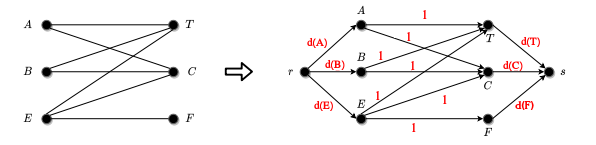
\includegraphics[width=40em]{digraph_deg.png}
  \captionsetup{labelformat=empty}
  \caption{Figure 11.1: digraph $D$ (on the right) created from an original graph $G$ (on the left)}
\end{figure}
Its is straightforward from the definition of $D$ that
\begin{align*}
\tag{11.1}
  \delta^\text{out}(\{r\}) &= \{(i, u) \in A : i = 1 \text{ and } u \in U\} = \{1\}\times U\\
  \tag{11.2}
  \delta^\text{in}(\{s\}) &= \{(i, w) \in A : i = 3 \text{ and } w \in W\} = \{3\}\times W
\end{align*}

We claim that
 \begin{align}
 \tag{11.3}
 \bar{u}(\delta^\text{out}(\{r\})) = d(U) \\
 \tag{11.4}
 \bar{u}(\delta^\text{in}(\{s\})) = d(W)
\end{align}


Indeed,
\begin{equation*}
\begin{aligned}
    \bar{u}(\delta^\text{out}(\{r\})) 
    &= \bar{u}(\{1\}\times U)) \\
    &= \sum_{a \in \{1\}\times U}{\bar{u}(a)} \\
    &= \sum_{u \in U}{\bar{u}((1, u))} \\
    &= \sum_{u \in U}{d(u)} \\
    &= d(U)
\end{aligned}
\end{equation*}

And analogously
\begin{equation*}
    \begin{aligned}
    \bar{u}(\delta^\text{in}(\{s\})) 
    &= \bar{u}(\{3\}\times W))  &&\text{(by 11.2)}\\
    &= \sum_{a \in \{3\}\times W}{\bar{u}(a)} \\
    &= \sum_{w \in W}{\bar{u}((1, w))} \\
    &= \sum_{w \in W}{d(w)} \\
    &= d(W)
    \end{aligned}
\end{equation*}


\begin{proposition} Restore the context from the exercise statement.

 Set $Z \coloneqq V \setminus (U \cup W)$.
 If $d(U) = d(W) = \frac{1}{2} d(V)$, then $d(Z) = 0$.
\end{proposition}
\begin{proof}
 Indeed, since $U$, $W$ and $Z$ are disjoint, we have
\begin{align*}
 V &= U \cup W \cup Z &\implies \\
 d(V) &= d(U) + d(W) + d(Z) &\implies \\
 d(V) &= \frac{1}{2} d(V) + \frac{1}{2} d(V) + d(Z) &\implies \\
 d(V) &= d(V) + d(Z) &\implies \\
 0 &= d(Z)
\end{align*}

\end{proof}


\newtheorem{lemma}{Lemma}
\begin{lemma}
    Restore the context from the exercise statement. Let $D \coloneqq (\{r, s\} \cup V, A, \psi)$ be a digraph and $\bar{u} : A \to \mathbb{R}_+$ be a capacity function as described above. Let $f$ be a maximum integral flow in $D$.
    
    Let $E' \coloneqq \{e \in E : f((2, e)) > 0 \}$ be (informally) the set of edges of $G$ with some flow in $D$ and let $H \coloneqq (V, E', \varphi\restr{E'})$ be a spanning subgraph of $G$.
    
    If $value(f) = d(U) = d(W) = \frac{1}{2} d(V)$, then $\deg_H = d$.
    
\end{lemma}
\begin{proof}

Let $v \in V$ be any vertex. There are 3 possible cases:

\textbf{Case 1: $v \in U$}.

The informal idea of this case is showing that the flow going inside of $v$ is $d(v)$, so by flow conservation the amount of flow going out is also $d(U)$, but the arcs that leaves $v$ with flow become the arcs of $H$, so $\deg_H = d(U)$. Now let us show this formally.

By (11.3) we have that $\bar{u}(\delta_D^\text{out}(\{r\})) = d(U) = value(f)$, so that $\delta_D^\text{out}(\{r\})$ is a minimum $rs$-cut in D.

Thus, Proposition 1 from Exercise 5 shows that
\begin{align*}
 \tag{11.5}
f(a) = \bar{u}(a)\text{, for each }a \in \delta^{\text{out}}(\{r\})
\end{align*}
And from this we get
\begin{align*}
 f((1, u)) &= \bar{u}((1, u)), \text{ for each } (1, u) \in \{1\} \times U &&\text{(by 11.5 and 11.1)}\\
  f((1, u)) &= \bar{u}((1, u)), \text{ for each } u \in U \\
\tag{11.6}
 f((1, u)) &= d(u), \text{ for each } u \in U &&\text{(by hypothesis)} 
\end{align*}

Now, from the construction of $D$, we have that the only arc entering any vertex $u \in U$ is the arc $(1, u)$, so 
\begin{align*}
 \tag{11.7}
 \delta_D^{\text{in}}(\{v\}) = \{(1, u)\}
\end{align*}
Again from the contruction of $D$, we have that the arcs leaving any vertex of $u \in U$ are those of the form $(2, e)$ such that $u$ was incident with $e$ in $G$.
So 
\begin{align*}
 \tag{11.8}
 \delta_D^{\text{out}}(v) = \{2\} \times \delta_G(v)
\end{align*}

The last facts we need are 
\begin{align*}
 \tag{11.9}
 \text{if } e \notin E' \text{, then } f((2, e)) = 0 \\
 \tag{11.10}
 \text{if } e \in E' \text{, then } f((2, e)) = 1 
\end{align*}
This is true because $f$ is integral and $\bar{u}((2,e)) = 1$, so $f((2, e))$ is either $0$ or $1$, and by definition it is $1$ if and only if $e \in E'$ .


Now, we can put everything together and get that

\begin{align*}
 d(v) 
 &= f((1, u)) &&\text{(by 11.6)}  \\
 &= f(\delta_D^{\text{in}}(v)) &&\text{(by 11.7)} \\
 &= f(\delta_D^{\text{out}}(v)) &&\text{(by flow conservation)} \\
 &= f(\{2\} \times \delta_G(v)) &&\text{(by 11.8)} \\
 &= f(\{2\} \times (\delta_G(v) \cap E')) &&\text{(by 11.9)} \\
 &= f(\{2\} \times (\delta_H(v))) \\ 
 &= \sum_{e \in \delta_H(v)}{f((2, e))} \\
 &= \sum_{e \in \delta_H(v)}{1} &&\text{(by 11.10)} \\
 &= |\delta_H(v)| \\
 &= \deg_H(v) \\
\end{align*}

\textbf{Case 2: }$v \in W$.

Since this exercise is already too long, and this case is analogous to the first one, we will only keep a more informal proof.


By (11.4) we have that $\bar{u}(\delta_D^\text{in}(\{s\})) = d(W) = value(f)$, so that $\delta_D^\text{in}(\{s\})$ is a minimum $rs$-cut in D. (Note that $\delta_D^\text{in}(\{s\})$ is an $rs$-cut because $\delta_D^\text{in}(\{s\}) = \delta_D^\text{out}(\{r\} \cup V)$).

Now, the next steps are analogous to case 1, just changing $\delta^{\text{in}}$ by $\delta^{\text{out}}$ and vice versa.
Doing this, we get that the amount of flow going out of $v$ is equal to $d(v)$, and it needs to be equal to the amount of flow going inside of $v$, and thus there are $d(v)$ arcs arriving at $v$ with some flow, and they will become the arcs of $H$.

So $\deg_H(v) = d(v)$

\textbf{Case 3: }$v \in V \setminus(U \cup W)$.

Since $G$ is $(U, W)$-bipartite and $v$ is not in $U$ nor $W$, there is no arc leaving $v$ in G, so there cant be any arc leaving $v$ in H.

And by Proposition 3, we got that $d(v) = 0$.

Hence $0 = d(v) = \deg_H(v)$.

Finally, in all three cases, $\deg_H(v) = d(v)$, so $\deg_H = d$.
\end{proof}
\begin{lemma}

    Restore the context from the exercise statement. Let $D \coloneqq (\{r, s\} \cup V, A, \psi)$ be a digraph and $\bar{u} : A \to \mathbb{R}_+$ be a capacity function as described in the begining of the exercise. 
    
    Let $f$ be a maximum integral $rs$-flow in $D$ (with respect to $\bar{u}$) and let $R \subseteq V$ be an optimal solution for (4.1) with input $(D, \bar{u}, r, s)$.
    
    Set $Z = V \setminus (U \cup W)$ and
    let $X \coloneqq (U \cap R) \cup (W \setminus R) \cup Z$. 
    
    If value$(f) < \frac{1}{2} d(V)$, then $|E[X]| < d(X) - \frac{1}{2} d(V)$.
\end{lemma}
\begin{proof}
First, because $U, W$ and $Z$ are disjoint, we have that
\begin{align*}
 \tag{11.11}
 d(X) = d(U \cap R) + d(W \setminus R) + d(Z)
\end{align*}

And for any two sets $B, C$ we have that
$B = (B \cap C) \cup (B \setminus C)$, thus
\begin{align*}
 \tag{11.12}
 d(U) = d(U \cap R) + d(U \setminus R) \\
 \tag{11.13}
 d(W) = d(W \cap R) + d(W \setminus R) \\
\end{align*}

Now, we claim that 
\begin{align*}
\tag{11.14}
\bar{u}(\delta_D^{\text{out}}(R)) = d(U \setminus R) + E[X] + d(W \cap R)
\end{align*}

If the arc $a$ is of the form $(1, u)$ then $a$ joins $r$ to $u$, so $a \in \delta_D^{\text{out}}(R)$ if and only if $u \notin R$.

If the arc $a$ is of the form $(2, e)$ then $a$ joins some $u \in U$ to some $w \in W$, so $a \in \delta_D^{\text{out}}(R)$ if and only if $u \in R$ and $w \notin R$, and in this case, by definition of X, $a \in E[X]$.

If the arc $a$ is of the form $(3, w)$ then $a$ joins some $w \in W$ to $s$, so $a \in \delta_D^{\text{out}}(R)$ if and only if $w \in R$.

This 3 cases shows that the sum of the capacities, by the definition of $\bar{u}$, is 

\begin{align*}
\bar{u}(\delta_D^{\text{out}}(R)) &= \bar{u}(U \setminus R) + \bar{u}(E[X]) + \bar{u}(d(W \cap R)) \\
&= d(U \setminus R) + E[X] + d(W \cap R)
\end{align*}

Finally, we can prove that
\begin{align*}
 E[X] &= \bar{u}(\delta_D^{\text{out}}(R) - d(U \setminus R) - d(W \cap R)) &&\text{(by 11.14)} \\
 &= value(f) - d(U \setminus R) - d(W \cap R)) &&\text{(R is optimal)} \\
 &= value(f) - d(U) + d(U \cap R) - d(W \cap R)) &&\text{(by 11.12)}\\
 &= value(f) - d(U) + d(U \cap R) - d(W) + d(W \setminus R)) &&\text{(by 11.13)}\\ 
 &= value(f) - d(U) + d(U \cap R) - d(W) + d(W \setminus R)) + d(Z) - d(Z)\\ 
 &= value(f) + d(X) - d(U) - d(W) - d(Z) &&\text{(by 11.11)} \\
 &= value(f) + d(X) - d(V) \\
 &< \frac{1}{2}d(V) + d(X) -d(V) &&\text{(by hypothesis)}\\ 
 &= d(X) -\frac{1}{2}d(V) \\  
\end{align*}
\end{proof}

Now, we can build our algorithm, and to solve the instance of the Max Flow problem, we will use the Edmonds-Karp Algorithm, because we know it satisfies our necessities.

\begin{algorithm}{}
\begin{algorithmic}[1]
\caption{Spanning Subgraph via Flows}
\Procedure{}{$G,U,W,d$} 
\State $A \gets U \sqcup E \sqcup W$ \Comment Define $D$ and $\bar{u}$ as in the beginning of the exercise
\State $D \gets (\{r, s\} \cup V, A, \psi)$
\For{$u \in U$}
        \State $\psi((1, u)) \gets (r, u)$
        \State $\bar{u}((1, u)) \gets d(u)$
      \EndFor
\For{$e \in E$}
        \State Let $\{u, w\} \coloneqq \varphi(e)$, with $u \in U$ and $w \in W$
        \State $\psi((2, e)) \gets (u, w)$ 
        \State $\bar{u}((2, e)) \gets 1$
      \EndFor
\For{$w \in W$}
        \State $\psi((1, u)) \gets (r, u)$
        \State $\bar{u}((1, u)) \gets d(u)$
      \EndFor
\State $(f, R) \gets$ EDMONDS-KARP($D, \bar{u}, r, s$)
\If{value$(f) = d(U) = d(W) = \frac{d(V)}{2}$}
\State $E' \gets \{e \in E : f((2, e)) > 0 \}$
\State $H \gets (V, E', \varphi\restr{E'})$
\State \textbf{return} $H$
\Else
\State $X \gets (U \cap R) \cup (W \setminus R) \cup (V \setminus (U \cup W))$ 
\State \textbf{return} $X$ 
\EndIf
\EndProcedure
\end{algorithmic}
\end{algorithm}

Lemma 1 shows that the spanning subgraph $H$ returned in line 18 is such that $\deg_H = d(H)$.

And if we get in the else of line 19, then at least one of the equalities of the if condition does not holds. In this case, we claim that value$(f) < \frac{d(V)}{2}$.

For this proof, we need to remember the weak duality relation that shows that 
\begin{align*}
\tag{11.15}
\text{value}(f) \leq \bar{u}(\delta_D^{\text{out}}(r)) = d(U) \\
\tag{11.16}
\text{value}(f) \leq \bar{u}(\delta_D^{\text{in}}(s)) = d() 
\end{align*}

If $d(U) < d(W)$, then we would have $2d(U) < d(U) + d(W) \leq d(V)$, so that $d(U) \leq \frac{d(V)}{2}$
So, indeed, value$(f) \leq d(U) < \frac{d(V)}{2}$.

If $d(W) < d(U)$, it is analogous.

And if $d(U) = d(W)$, we have that in the case of value$(f) = d(U)$, then the equalitie value$(f) = \frac{d(V)}{2}$ is the one that does not hold. So the inequality value$(f) = d(U) \leq \frac{d(V)}{2}
$ implies value$(f) < \frac{d(V)}{2}$.
In the other case, value$(f) < d(U) \leq \frac{d(V)}{2}$.

Hence in all cases value$(f) < \frac{d(V)}{2}$, thus Lemma 2 garantees that the set $X$ returned in line 21 satisfies the condition we expected.

\blankpage

\section*{Exercise 19}

We will assume that $D$ has no parallel arcs, because parallel arcs play no role while dealing with vertex-disjoint paths.

We will create an auxiliar digraph, that splits each vertex into to vertices, one where there are arcs only arrive, and the other where the arcs only leave, these two connected by one new arc.

Let $D' \coloneqq (V', A', \varphi'$), where
$$ V' = \{0, 1\} \times V \text{, where we denote } v_i \coloneqq (i, v)$$
$$ A' = V \sqcup A $$
$$ \varphi' : A' \to V' \times V' \text{ defined by } $$
$$ \varphi'((i, x)) \coloneqq 
\left\{
	\begin{array}{ll}
		(x_0, x_1) & \mbox{if } i = 1 \text{, } x \in V \\
		(v_1, w_2) & \mbox{if } i = 2 \text{, } x \in A \text{, where } \varphi(x) = (v, w) \\
	\end{array}
\right. 
$$

Let $u : A' \to \mathbb{R}_+$ be a capacity function defined by $u(a) = 1$ for each $a \in A'$.

Let $f$ be a maximum integral flow in $D'$ with respect to $u$, let $D'(f, u)$ be the residual digraph defined as in 14.3 from the lectures, and let $R \coloneqq \{v \in V : r \rightsquigarrow_{D'(f, u)} v \}$ be the set of vertices reacheable from $r$ in the residual digraph.

We may think that $(f, R)$ is the pair returned by Edmonds-Karp Algorithm with input $(D', u, r, s)$.

From theorem 14.9, we have that $R$ is an optimal solution for the minimum capacity $rs$-cut problem.

Now, our strategy will be decompose $f$ in $rs$-paths and show that these paths are pairwise internally vertex-disjoint. 

By exercise 18.10 (Decomposition of flows), we have that there is a set  $\mathcal{C}$ of cycles and a set $\mathcal{P}$ of $rs$-paths in $D'$  such that (for some $y \in \mathbb{R}_+^{\mathcal{C}}$ and $x \in \mathbb{R}_+^{\mathcal{P}}$)
$$f = \sum_{C \in \mathcal{C}}{y_C\mathbbm{1}_C} + \sum_{P \in \mathcal{P}}{x_P\mathbbm{1}_P}$$

But we have that there is no $(r, s)$ arc in $A$, so that there can not be any $(r_i, s_i)$ arc in $A'$, then there is no $rs$-cycle composing the flow.

And since $f$ is integral, we can take $x$ integral, but then we have that $x = \mathbbm{1}$, because $f(a)$ is either 0 or 1, for any $a \in A'$. (And if $f = 0$ then there is no $rs$-path) 

Then, the flow we obtained can be written as a collection of $rs$-paths. 

Now, for each $v \in V$, there is only one arc joining $v_0$ and $v_1$ in $D'$, and this arc has capacity 1.

Then, for any two paths $P_1, P_2$ in $\mathcal{P}$, we have that $P_1$ and $P_2$ are internally vertex-disjoint. Because if there was a vertex $v_i \in V(P_1) \cap V(P_2)$, then the arc $a \coloneqq (1, v)$ should carry at least two units of flow (one from $P_1$ and the other from $P_2$), but then $f$ would not be feasible, because $f(a) \geq 2 > 1 = u(a)$. 

Note that value$(f) = |\mathcal{P}|$, because each unit of flow needs to come from a different path.

So, for any flow $f$ we can obtain a set of internally vertex-disjoint paths.

Now, define $U \coloneqq \{v \in V' : $ there is $w \in V$ and $a \in \delta^{\text{out}}(R) $ with $\varphi'(a) = (v, w)\}$ as the set of vertices in the ``frontier'' of $R$.

The next step is to verify that $U$ is a minimum sized $rs$-vertex cut in $D'$.

Note that any $rs$-path $P$ in $D'$ need to carry some flow, if it doesn't, then $f$ would not be maximum, because we could send more flow using $P$.

Now, by Proposition 1 from exercise 5, every arc leaving $U$ is with full capacity (because they are the ones in $\delta^{\text{out}}(R))$), i.e., $f(a) = u(a) = 1$, and we have that   
$|U| = |\delta^{\text{out}}(R)| = u(\delta^{\text{out}}(R)) = $ value$(f)$ = $|\mathcal{P}|$, so each vertex in $U$ is part of one and only one $rs$-path.

Thus, indeed, we can extend the strong complementary slackness propertie between $f$ and $R$ to $\mathcal{P}$ and $U$.

\end{document}
